% ===========================================================================
%  Minkowski Kart: A relativistic kart-racing game extending OpenRelativity
%
%  Manuscript prepared for submission to the American Journal of Physics.
%  Uses REVTeX 4.2 with the AIP/AJP options (compile with pdflatex; run twice,
%  then bibtex, then pdflatex twice more, to resolve references).
% ===========================================================================
\documentclass[aip,amsmath,amssymb,reprint,nofootinbib]{revtex4-2}

\usepackage{graphicx}
\usepackage{bm}
\usepackage{xcolor}
\usepackage{listings}
\usepackage{tikz}
\usetikzlibrary{arrows.meta,calc,decorations.pathmorphing}
\usepackage{pgfplots}
\pgfplotsset{compat=1.16}
\usepackage[colorlinks=true,allcolors=blue]{hyperref}

% ---- a compact code-listing style for the short GLSL/C++ excerpts ----------
\lstdefinestyle{mk}{
  basicstyle=\ttfamily\footnotesize,
  keywordstyle=\color{blue!60!black},
  commentstyle=\color{green!40!black}\itshape,
  numberstyle=\tiny\color{gray},
  breaklines=true,
  showstringspaces=false,
  frame=single,
  columns=fullflexible,
}
\lstset{style=mk}

\begin{document}

\title{Minkowski Kart: A relativistic kart-racing game\\ extending the OpenRelativity project}

\author{R.~Christie}
\email{slipperyfish223@gmail.com}
\affiliation{Independent researcher}
% NOTE: add co-authors / institutional affiliation before submission.

\date{\today}

\begin{abstract}
We present \emph{Minkowski Kart}, an open-source arcade kart-racing game in which
special-relativistic kinematics, optics, and dynamics are woven into ordinary
gameplay. The game is built on the SuperTuxKart engine and borrows its
relativistic visual model from the MIT Game Lab's \emph{OpenRelativity} toolkit,
which popularised real-time relativistic rendering for the games \emph{A Slower
Speed of Light} and its successors. We describe three substantive extensions of
that work. First, the apparent position of every object is computed from the
\emph{retarded} (emission-time) light-travel solution combined with relativistic
aberration of the incoming ray, rather than from an instantaneous Lorentz
contraction of static world geometry; this Terrell--Penrose construction is
applied per object, so independently moving karts and projectiles each warp
according to their own velocity. Second, because the apparent-position map is
strongly nonlinear, we introduce \emph{dynamic GPU mesh tessellation}: hardware
tessellation-control and -evaluation shaders adaptively subdivide track and
object geometry at render time, with the subdivision density driven both by
proximity to the player and by a closed-form estimate of the local magnification
produced by aberration. This removes the faceting and surface-clipping artefacts
that otherwise force authors to ship pre-subdivided meshes. Third, the
relativistic effects are made \emph{playable}: a user-adjustable speed of light,
a relativistic longitudinal mass that scales the engine force by $1/\gamma^3$,
proper-time accumulation, and a suite of physics-themed power-ups (warp bubble,
time dilation, anti-particle pair production, wormholes, gravitational-wave
fronts) turn relativistic phenomena into game mechanics. We discuss the
implementation, the pedagogical affordances of an interactive low-$c$ world, and
the limitations of the approach.
\end{abstract}

\maketitle

% ===========================================================================
\section{Introduction}
% ===========================================================================

Special relativity is notoriously difficult to build intuition for, precisely
because its effects are imperceptible at everyday speeds. A productive teaching
strategy is therefore to lower the speed of light $c$ until relativistic effects
dominate the visible world, and to let students move through that world
interactively.\cite{Savage2007,Kraus2008} The most influential modern
realization of this idea is the MIT Game Lab's \emph{OpenRelativity}
toolkit\cite{Sherin2016} and the game \emph{A Slower Speed of Light}, in which a
first-person player walks through a static environment whose apparent geometry
and color are transformed in real time as the in-game $c$ is gradually reduced
toward the player's running speed. OpenRelativity is distributed as a Unity
plugin\cite{OpenRelativityRepo} and has been widely adopted for classroom
demonstrations and outreach.

OpenRelativity makes two simplifying assumptions that are well suited to its
walking-simulator setting but limiting for a fast, multi-object arcade game.
\emph{(i)} The relativistic vertex transform is applied to a \emph{static} world
in the player's instantaneous rest frame: the player is treated as moving
through fixed scenery, and there is no general mechanism for many independent
objects to each carry their own velocity into the optical transform. \emph{(ii)}
The transform is evaluated only at existing mesh vertices, so faithful rendering
requires geometry that is already finely subdivided; coarse meshes visibly
facet because the nonlinear warp is interpolated linearly across large
triangles.

We should be clear about what is and is not new here. The underlying optical
model---placing each object at its retarded (light-emission) position and
aberrating the incoming ray into the observer's frame---is the standard
``photographic'' approach to relativistic visualization, developed over several
decades and used, in one form or another, by essentially all of the prior
art.\cite{Hsiung1990,Weiskopf2000,Kraus2008,Savage2007,Sherin2016} The
Terrell--Penrose insight that this produces apparent \emph{rotation} rather than
visible contraction is older still.\cite{Terrell1959,Penrose1959,Weisskopf1960}
Our contribution is not a new optical model but an engine architecture that makes
that model work in a fast, many-body, competitively played game on
externally-authored content. Concretely, the novel elements are (a) applying the
retarded-time/aberration transform \emph{per object}, each with its own velocity,
so independently moving karts and projectiles warp correctly relative to a moving
observer; (b) a dynamic GPU tessellation scheme whose subdivision density is
driven by a closed-form estimate of the local aberration magnification, which lets
the nonlinear warp render cleanly on arbitrary track geometry; and (c) a playable
relativistic \emph{dynamics} layer (adjustable $c$, $1/\gamma^3$ longitudinal
response, proper-time accounting, velocity clamping) that turns the effects into
game mechanics rather than a passive visual overlay.

\emph{Minkowski Kart} is an open-source game that keeps OpenRelativity's
physical model and even reuses its spectral Doppler-shift code, but rebuilds the
relativistic pipeline around the demands of a racing game: dozens of objects
moving at appreciable fractions of $c$ relative to one another, on artist-authored
tracks of arbitrary tessellation, rendered through two graphics backends
(OpenGL and Vulkan). The game is a fork of
SuperTuxKart\cite{STK}, an established open-source kart racer, and is released
under the GPLv3.

This paper documents the physics model and the three principal extensions over
OpenRelativity: a per-object retarded-time/aberration optical model
(Sec.~\ref{sec:optics}), dynamic GPU mesh tessellation driven by the local
nonlinearity of the warp (Sec.~\ref{sec:tessellation}), and a set of relativistic
\emph{dynamics} that make the effects controllable as gameplay
(Sec.~\ref{sec:dynamics}). We also describe the relativistic power-up system
(Sec.~\ref{sec:game}) and the Doppler/searchlight color shift
(Sec.~\ref{sec:doppler}), and we close with pedagogical observations and
limitations.

% ===========================================================================
\section{The game}\label{sec:game}
% ===========================================================================

Minkowski Kart plays as a conventional arcade kart racer: the player drives a
kart around a closed circuit, collects power-up boxes, and competes against
human or AI opponents. What differs is that the in-game speed of light is small
enough to be reached during normal driving. The default coordinate speed of
light is $c = 35$~u/s (game units per second; roughly the top speed of a boosted
kart), and the player may set it anywhere in the range $15$--$1000$~u/s
from the ``Relativity'' options menu, with a hard cap on coordinate speed at
$\beta_{\max} = 0.98$ by default. As a kart approaches $c$, opponents and scenery
visibly distort, their colors Doppler-shift, and the player's own clock runs slow
relative to coordinate time.

\begin{figure}[t]
\centering
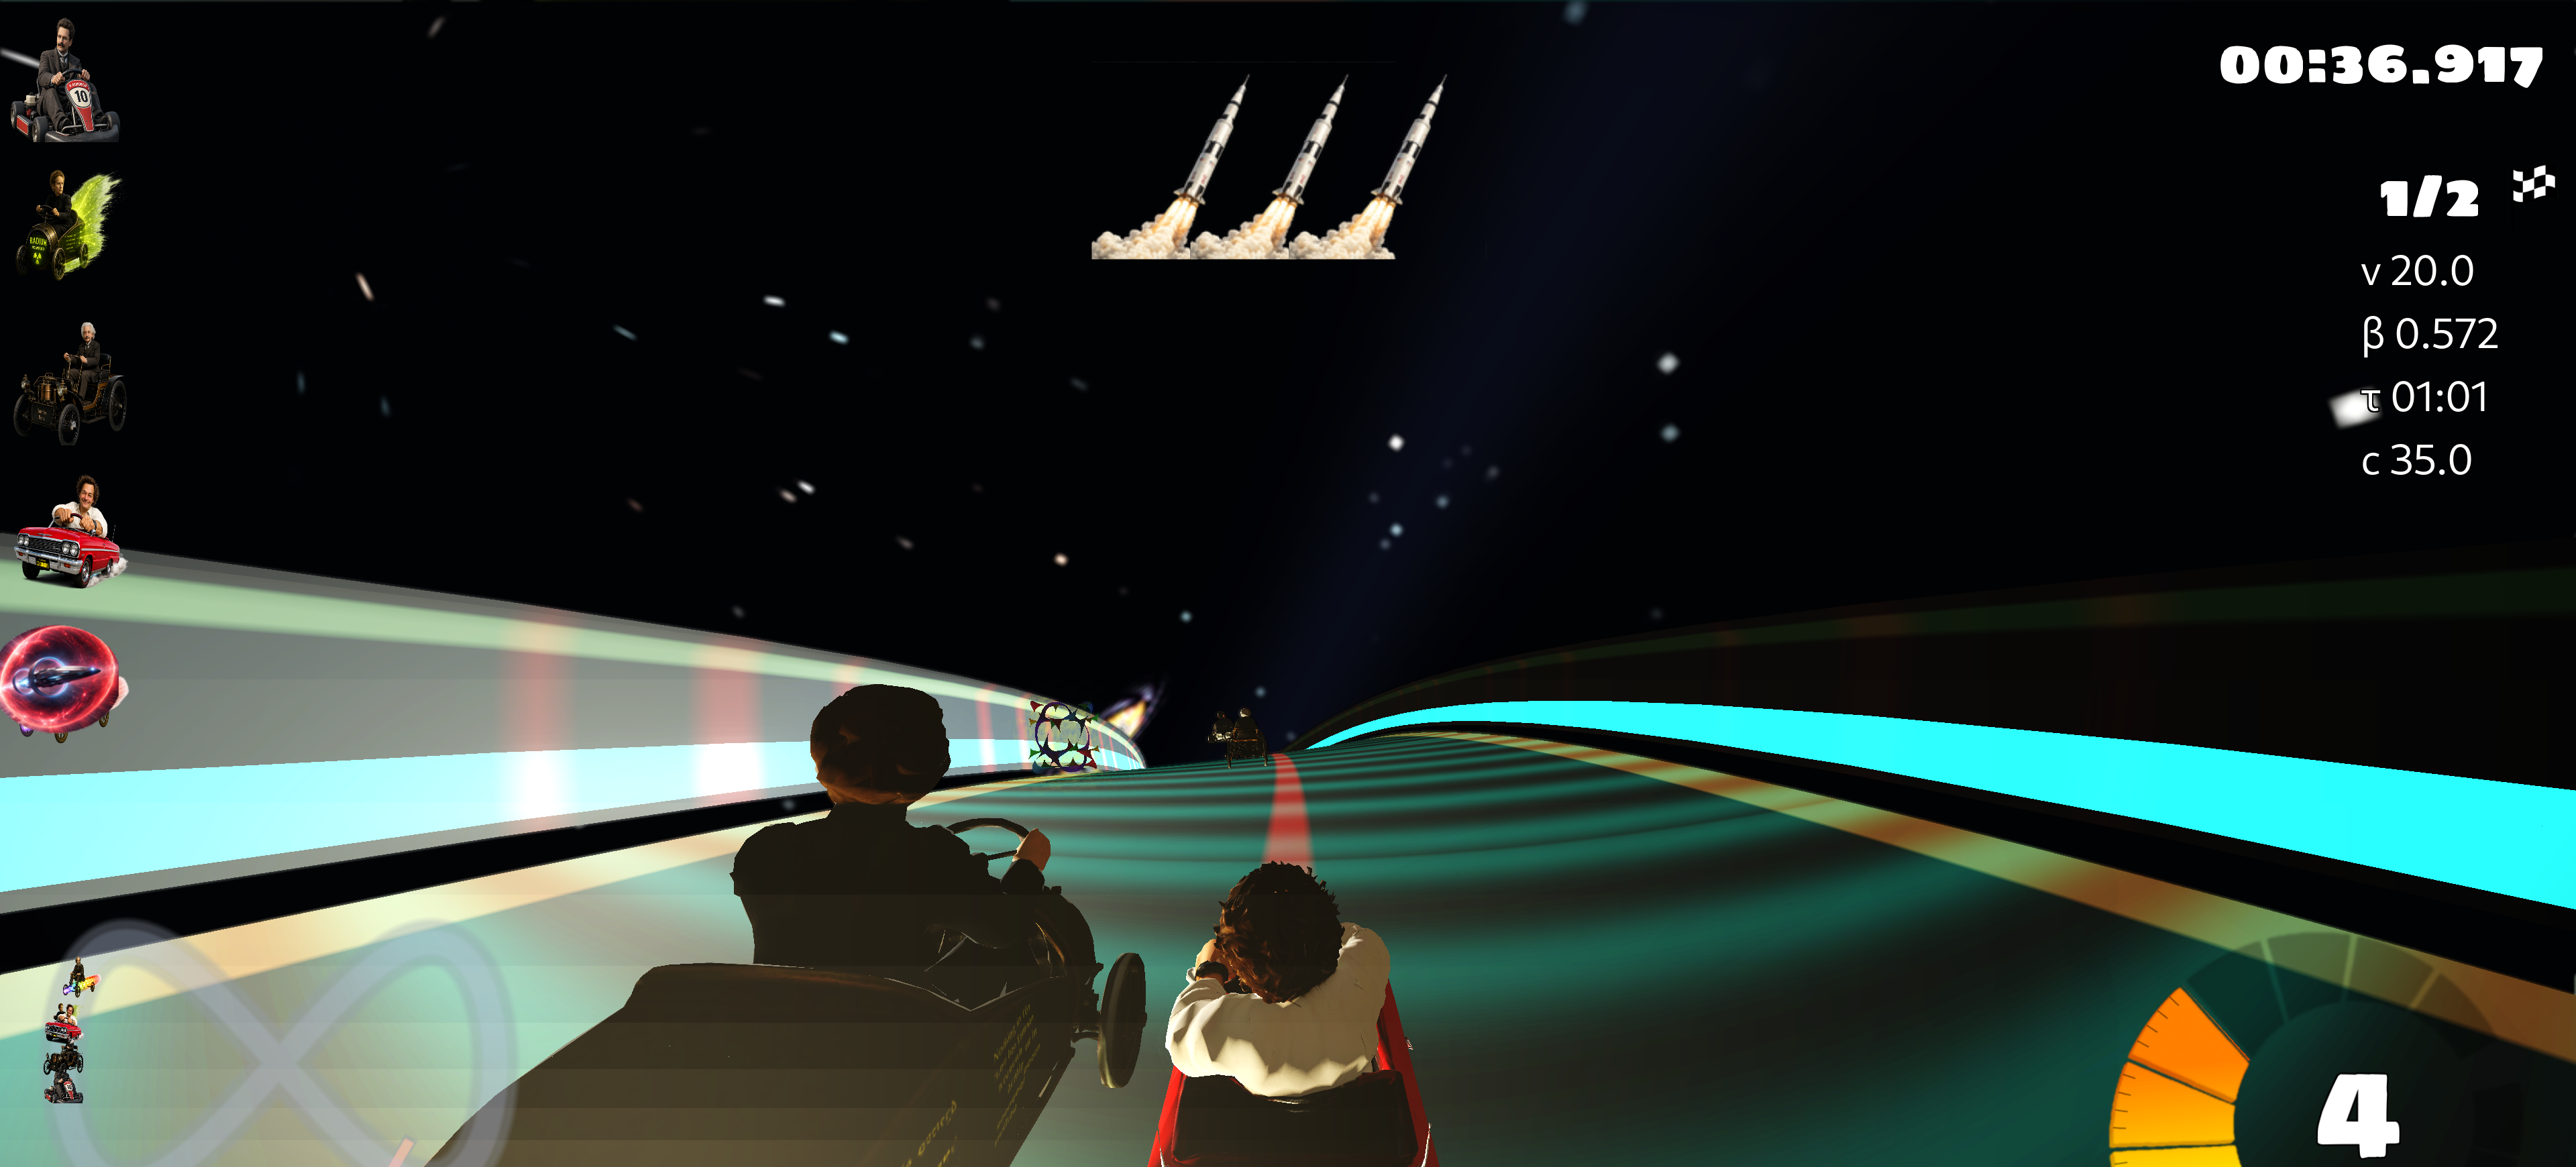
\includegraphics[width=\columnwidth]{figures/mobius_race_hud.png}
\caption{An all-AI race on the M\"obius Trip track. The heads-up display reports
the live relativistic telemetry of the lead kart---coordinate speed $v$, the
ratio $\beta=v/c$, accumulated proper time $\tau$, and the in-game speed of light
$c$. Even at $\beta\approx0.57$ the track surface and trailing opponents are
already visibly warped by aberration and retarded-time displacement
(Sec.~\ref{sec:optics}).}
\label{fig:race}
\end{figure}

Each power-up is themed on a relativistic or particle-physics concept
(Table~\ref{tab:items}), so that the act of using an item is also an encounter
with the idea behind it. The game runs on desktop (Windows, Linux, macOS) and
supports online multiplayer in which the relativistic rules---$c$, $\beta_{\max}$,
and the power-up boost multiplier---are set by the server and synchronized to all
clients.

\begin{table}[t]
\caption{Representative relativistic power-ups. The full item logic lives in
\texttt{src/items/} and item weights in \texttt{data/powerup.xml}.}
\label{tab:items}
\begin{ruledtabular}
\begin{tabular}{ll}
Power-up & Physical motif \\
\hline
Warp Bubble    & Local boost to $c$ ($10\times$ normal) and shield \\
Black Hole     & Homing mass with lensing and orbital capture \\
Wormhole       & Linked pair of traversable spacetime portals \\
Time Dilation  & Expanding wavefront that lowers others' $c$ \\
Anti-Karticle  & Mirror clone; annihilates in a pair-production flash \\
Super Position & Global spacetime ``collapse'' and world pulse \\
Photon         & High-speed tether / Doppler blast \\
Maxwell--Boltzmann & Gaussian velocity kicks aimed at the leader \\
\end{tabular}
\end{ruledtabular}
\end{table}

% ===========================================================================
\section{Relativistic kinematics with an adjustable \texorpdfstring{$c$}{c}}
\label{sec:kinematics}
% ===========================================================================

All relativistic bookkeeping is centralized in a single module
(\texttt{src/relativity/relativity\_math.cpp}). For a kart with signed speed $v$
along its motion and an effective speed of light $c$, the standard invariants

\begin{equation}
\beta = \frac{|v|}{c}, \qquad
\gamma = \frac{1}{\sqrt{1-\beta^2}}
\end{equation}

are clamped to $\beta < 1$ for numerical safety. Proper time is accumulated each
physics tick from the coordinate time step $\Delta t$ as

\begin{equation}
\Delta\tau = \frac{\Delta t}{\gamma},
\label{eq:propertime}
\end{equation}

so each kart carries both a coordinate clock and a proper clock; the running
difference is the twin-paradox bookkeeping made literal. The speed of light is
not a fixed constant but a smoothly ramped state variable: when a power-up
changes a kart's local $c$ (for example the warp bubble, which sets it to
$10\times$ the baseline), the value eases over ${\sim}1$~s with a smoothstep
so that the optical distortion does not snap discontinuously.

% ===========================================================================
\section{Optics: retarded position and aberration}\label{sec:optics}
% ===========================================================================

\begin{figure*}[t]
\centering
\begin{tikzpicture}
\node[anchor=south west,inner sep=0] (img)
  {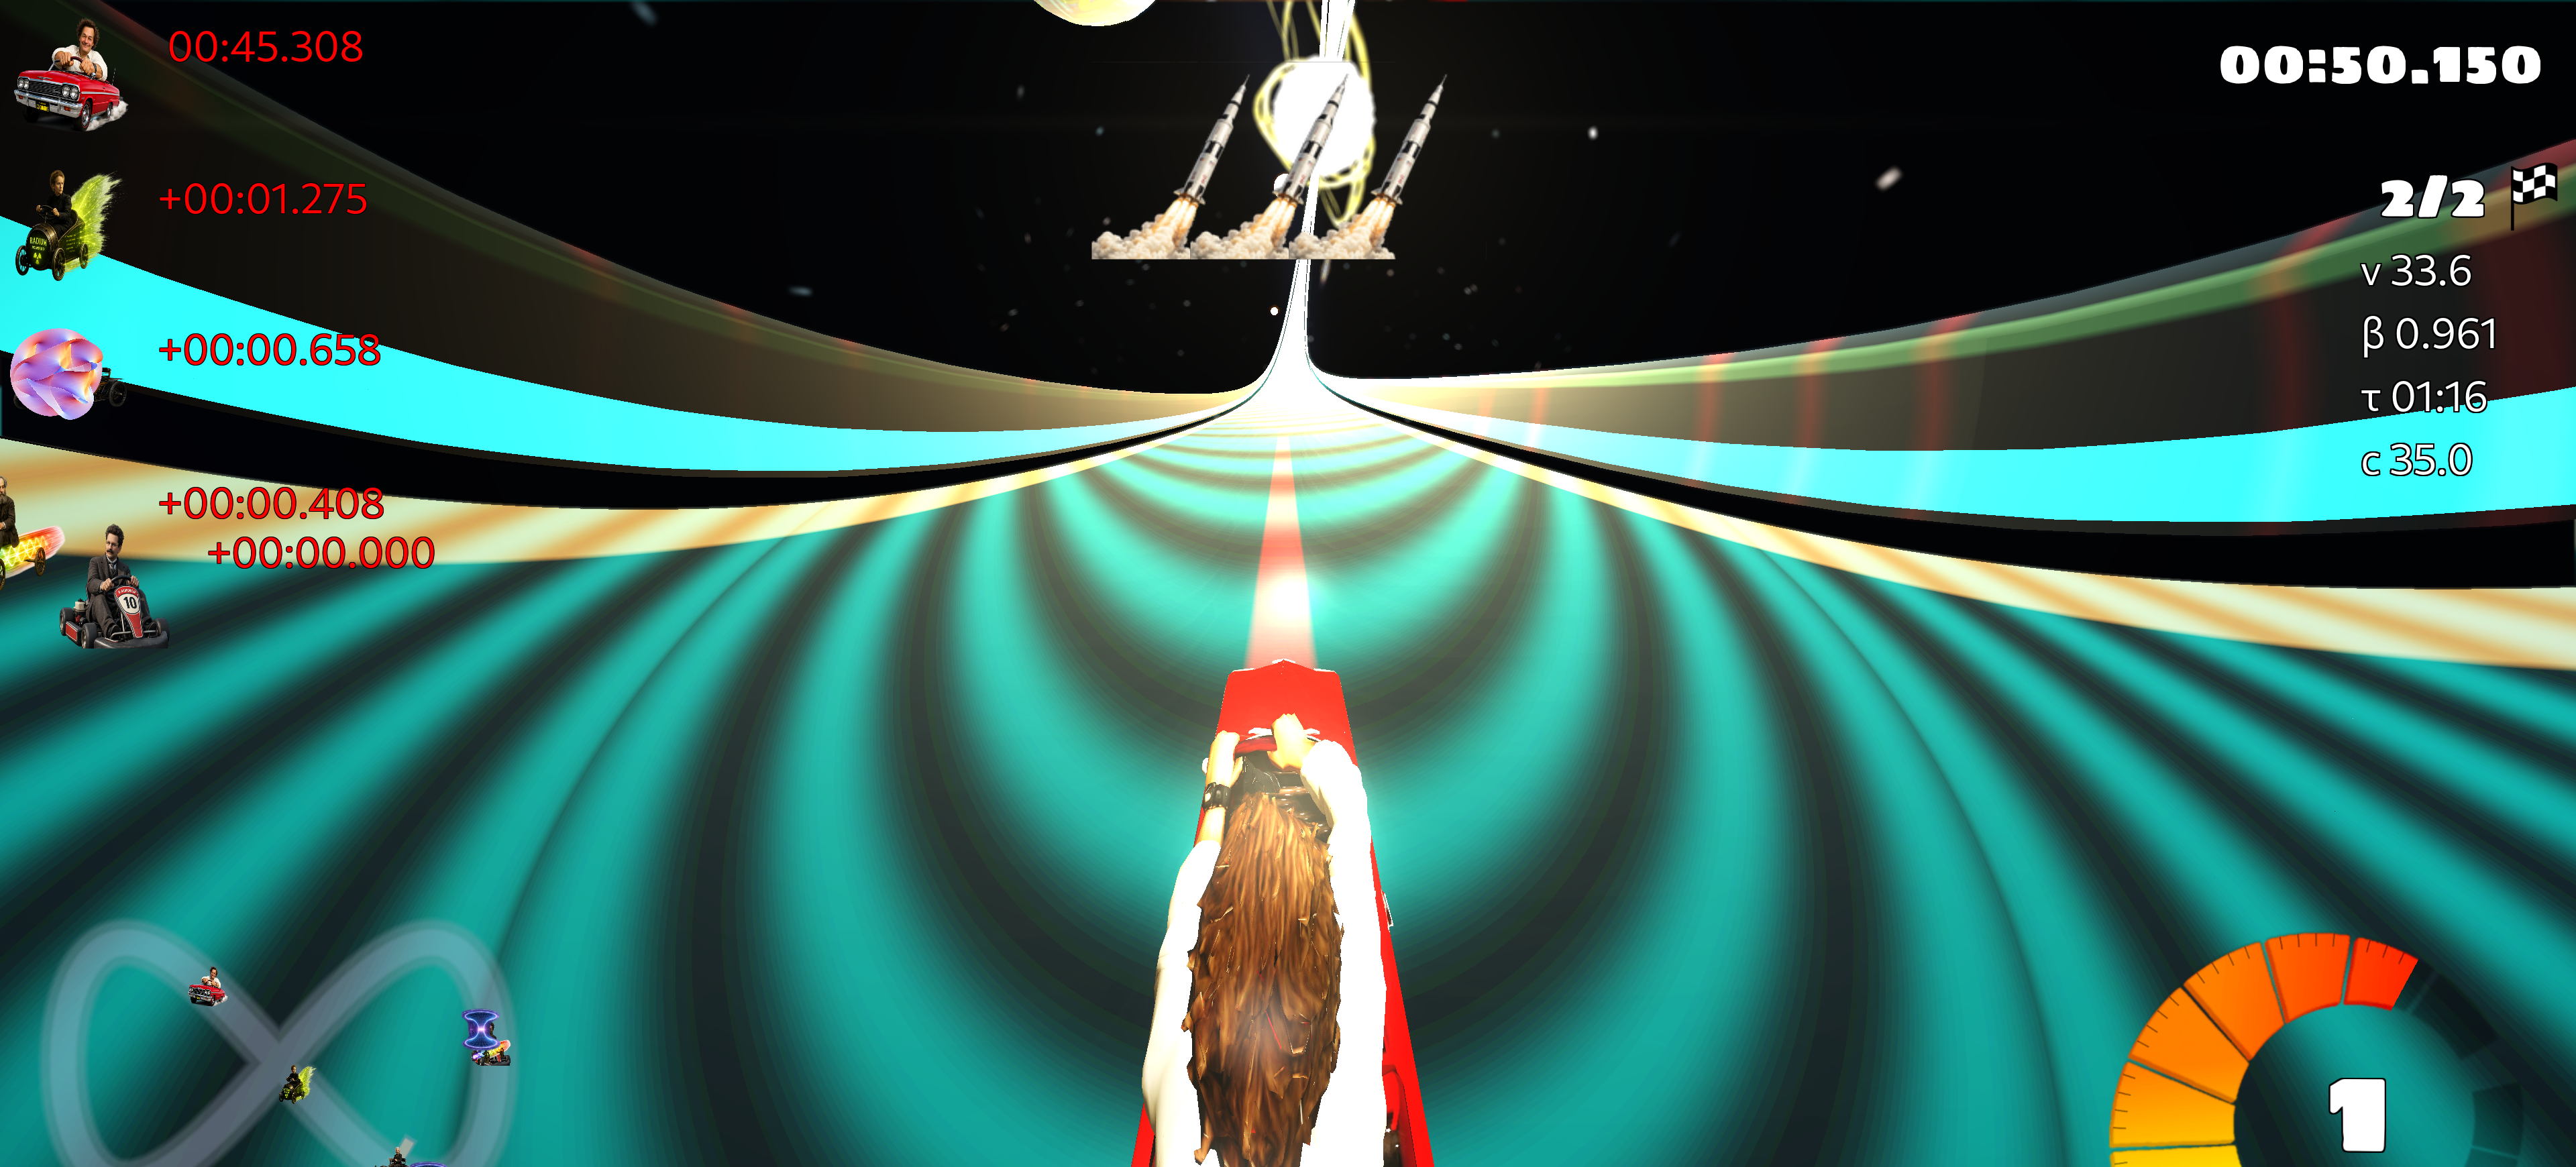
\includegraphics[width=0.92\textwidth]{figures/mobius_high_beta_warp.png}};
\begin{scope}[x={(img.south east)},y={(img.north west)},
              font=\footnotesize\sffamily,
              every node/.style={text=white}]
  \draw[-{Stealth[length=2mm]},white,thick]
    (0.30,0.78) node[anchor=east,align=right]{forward aberration\\cone (Eq.~\ref{eq:aberration})}
    -- (0.50,0.62);
  \draw[-{Stealth[length=2mm]},white,thick]
    (0.27,0.30) node[anchor=east,align=right]{Doppler-shifted\\track (Eq.~\ref{eq:doppler})}
    -- (0.45,0.33);
\end{scope}
\end{tikzpicture}
\caption{Strong relativistic distortion at $\beta=0.961$ ($\gamma\approx3.7$) on
the M\"obius Trip track. Forward aberration squeezes the entire forward
hemisphere into a narrow cone ahead of the kart (the ``headlight'' effect of
Eq.~\eqref{eq:aberration}), bowing the straight track into concentric arcs, while
the relativistic Doppler/searchlight shift of Eq.~\eqref{eq:doppler} paints the
surface in shifted bands (Sec.~\ref{sec:doppler}). The geometry is resolved
without faceting because the track is dynamically tessellated on the GPU
(Sec.~\ref{sec:tessellation}). The HUD reads $v=33.6$, $\beta=0.961$, $c=35$.}
\label{fig:warp}
\end{figure*}

The central visual question is: where does an object \emph{appear} to a moving
observer? Minkowski Kart answers it the same way a camera does, in two steps,
and---unlike OpenRelativity's contraction-of-static-geometry approach---it
applies the construction to each object using that object's own velocity.

\paragraph{Retarded (emission-time) position.}
Light reaching the observer now was emitted in the past, when the object was
elsewhere. For an object at relative position $\bm{r}$ moving with velocity
$\bm{u}$, the emission time offset $\Delta t_e \le 0$ satisfies
$|\bm{r} + \bm{u}\,\Delta t_e| = -c\,\Delta t_e$, i.e.\ the quadratic

\begin{equation}
(\bm{u}\!\cdot\!\bm{u} - c^2)\,\Delta t_e^{\,2}
+ 2(\bm{r}\!\cdot\!\bm{u})\,\Delta t_e
+ \bm{r}\!\cdot\!\bm{r} = 0 .
\label{eq:retarded}
\end{equation}

We take the most-recent past root and displace the object to its
emission-time position $\bm{r}' = \bm{r} + \bm{u}\,\Delta t_e$. This is the
geometric origin of the Terrell--Penrose effect: because near and far parts of a
fast object emitted the light reaching the eye at different times, a passing
object appears \emph{rotated} rather than merely contracted.\cite{Terrell1959,Penrose1959}

\paragraph{Aberration of the incoming ray.}
The direction $\hat{\bm{d}}$ of the emission-time ray is then transformed from
the world frame into the observer's frame by the relativistic aberration map,
which for an observer with velocity $\bm{\beta}c$ and Lorentz factor $\gamma$
beams forward rays toward the direction of motion (the ``headlight'' effect):

\begin{equation}
\hat{\bm{d}}_{\mathrm{obs}}
= \frac{\dfrac{1}{\gamma}\hat{\bm{d}}
  + \left[\dfrac{\gamma}{\gamma+1}(\bm{\beta}\!\cdot\!\hat{\bm{d}}) + 1\right]\bm{\beta}}
  {1 + \bm{\beta}\!\cdot\!\hat{\bm{d}}} .
\label{eq:aberration}
\end{equation}

The apparent position is finally $\bm{p}_{\mathrm{obs}} =
\bm{p}_{\mathrm{eye}} + |\bm{r}'|\,\hat{\bm{d}}_{\mathrm{obs}}$.

A deliberate design choice---documented in the shader source---is that
\emph{no explicit Lorentz contraction} is applied to positions, normals, or
tangents. What a camera records is fully captured by the retarded position plus
aberration; coordinate length contraction is a statement about simultaneity in a
chosen frame, and adding it on top of the optical transform would double-count
the effect.\cite{Weisskopf1960} Lighting is therefore evaluated with unmodified
world-space normals, because light transport happens in the world frame.

Equations \eqref{eq:retarded}--\eqref{eq:aberration} are implemented identically
on the CPU (for gameplay queries such as ``where does the track surface appear?''
used by the anti-clipping logic) and on the GPU (for rendering), so the two never
disagree. The GPU version lives in
\texttt{data/shaders/utils/relativity\_visual.vert} and is included by every
relativistic vertex/tessellation stage:

\begin{lstlisting}[language=C]
// per-vertex apparent position (GLSL, abridged)
relative = world_position - u_observer_pos;
relative = retardedEmissionPosition(relative, object_velocity);
vec3 d_obs = worldDirToObserverDir(normalize(relative));
return u_observer_pos + length(relative) * d_obs;
\end{lstlisting}

% ===========================================================================
\section{Dynamic mesh tessellation}\label{sec:tessellation}
% ===========================================================================

The apparent-position map of Sec.~\ref{sec:optics} is strongly nonlinear in
world position. If it is evaluated only at the corners of a coarse triangle and
then interpolated linearly across the face---as it is when a static vertex shader
warps an artist's mesh---straight edges that should bow become visibly faceted,
and the warped track surface develops cracks and clips through karts. In
OpenRelativity this is handled by authoring heavily subdivided geometry. That is
impractical for a racing game whose tracks are large, externally authored, and
shared with the non-relativistic engine.

Minkowski Kart instead subdivides geometry \emph{dynamically on the GPU} at
render time, using the hardware tessellation stages
(\texttt{data/shaders/sp\_tess.tesc} and \texttt{sp\_tess.tese}). The
tessellation-control shader assigns each triangle edge a subdivision level, and
the tessellation-evaluation shader re-applies the relativistic apparent-position
map \eqref{eq:retarded}--\eqref{eq:aberration} at every newly generated vertex,
so the warp is sampled where it is actually nonlinear instead of being
interpolated across it.

\paragraph{Distance-adaptive base level.}
The base subdivision keeps the rendered edge length below a target. Rather than
cutting tessellation off at a fixed radius (which leaves large, rigidly warped
triangles in the distance), the target edge length \emph{grows} with distance
from the player, so geometry keeps subdividing everywhere, just more coarsely far
away:
\begin{equation}
\ell_{\mathrm{target}}(d) = \ell_0 \,\max\!\left(1,\ \frac{d}{R_0}\right)
\Big/\, A(\bm{\beta}),
\label{eq:target}
\end{equation}
with near-field target $\ell_0 = 0.1$, falloff scale $R_0 = 10$ world units, and
the tessellation level for an edge of length $\ell$ taken as
$\mathrm{clamp}(\ell/\ell_{\mathrm{target}},\,1,\,64)$.

\paragraph{Aberration-aware amplification.}
The factor $A(\bm{\beta})\ge 1$ in Eq.~\eqref{eq:target} is the novel ingredient.
Aberration magnifies image space anisotropically: rays \emph{behind} a forward-moving
observer are spread out by a factor $\sim 1/(1+\bm{\beta}\!\cdot\!\hat{\bm{d}})$, so
geometry there must be subdivided more finely to keep the warp smooth. We estimate
the local magnification directly from the edge midpoint direction $\hat{\bm{d}}$:
\begin{equation}
A(\bm{\beta}) = \mathrm{clamp}\!\left(
  \frac{1}{\max(1+\bm{\beta}\!\cdot\!\hat{\bm{d}},\,\tfrac18)},\ 1,\ 8\right).
\label{eq:amp}
\end{equation}
This raises the subdivision density precisely where the optical transform is most
expansive (behind the kart at high $\beta$) and relaxes it elsewhere, spending the
tessellation budget where the eye can see the difference.

\paragraph{Crack-free guarantee.}
Both Eq.~\eqref{eq:target} and Eq.~\eqref{eq:amp} depend \emph{only on the two
endpoints of an edge} (and on global observer state), never on the interior or
the opposite vertex of a triangle. Two triangles that share an edge therefore
compute exactly the same level for it, and the tessellator produces matching
vertices on both sides---so no T-junction cracks appear along shared edges, a
property that is otherwise easy to violate with adaptive tessellation.

\begin{figure}[t]
\centering
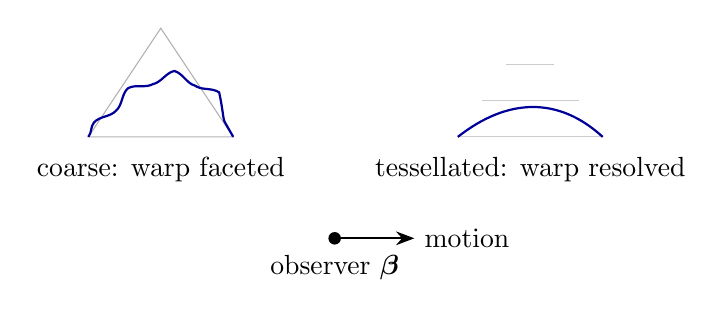
\begin{tikzpicture}[scale=0.92,>=Stealth]
  % observer
  \node[circle,fill=black,inner sep=1.6pt,label=below:{observer $\bm{\beta}$}] (O) at (0,0) {};
  \draw[->,thick] (O) -- (1.1,0) node[right]{motion};
  % coarse triangle (left, faceted)
  \begin{scope}[xshift=-3.4cm,yshift=1.4cm]
    \draw[gray!60] (0,0) -- (2,0) -- (1,1.5) -- cycle;
    \draw[thick,blue!60!black,decorate,decoration={snake,amplitude=1.6pt,segment length=6mm}]
      (0,0) .. controls (0.7,0.9) and (1.4,1.0) .. (2,0);
    \node at (1,-0.45) {coarse: warp faceted};
  \end{scope}
  % fine triangle (right, smooth)
  \begin{scope}[xshift=1.7cm,yshift=1.4cm]
    \foreach \i in {0,...,3}{
      \draw[gray!40] (0,0) -- (2,0);
      \draw[gray!40] ($(0,0)!{\i/3}!(1,1.5)$) -- ($(2,0)!{\i/3}!(1,1.5)$);
    }
    \draw[thick,blue!60!black] (0,0) .. controls (0.7,0.55) and (1.4,0.55) .. (2,0);
    \node at (1,-0.45) {tessellated: warp resolved};
  \end{scope}
\end{tikzpicture}
\caption{Schematic of dynamic tessellation. The nonlinear apparent-position warp
(blue) is poorly captured across a coarse triangle (left) but well resolved once
the triangle is adaptively subdivided on the GPU and the warp is re-evaluated at
the new vertices (right). Subdivision density rises with proximity to the
observer and with the aberration magnification $A(\bm{\beta})$ of
Eq.~\eqref{eq:amp}.}
\label{fig:tess}
\end{figure}

\paragraph{Where it matters.}
The benefit of dynamic tessellation scales with the size of the base triangles
relative to the curvature of the warp: it is dramatic on coarse or distant
geometry---a large ground or water plane subdivided into a handful of huge
triangles will visibly facet and clip without it---and negligible on geometry
that is already finely authored. On a tightly subdivided track such as the
M\"obius Trip circuit used for our figures, disabling tessellation leaves the
warped surface nearly indistinguishable even under magnification, because the
artist's mesh is fine enough to sample the warp adequately on its own. The point
of the adaptive scheme is precisely that the engine need not assume either case:
it spends subdivision only where the local triangle size and the aberration
magnification of Eq.~\eqref{eq:amp} demand it, so the same renderer handles a
coarse hand-made plane and a dense imported mesh without per-asset tuning.

\paragraph{Other anti-clipping modes.}
Tessellation is one of several user-selectable strategies for reconciling the
warped visual surface with the unwarped collision mesh. The Relativity menu also
exposes a cheap height-correction mode (adjusting visual height against the
physical track), a tangent-velocity-projection mode, and a combined
``tessellation $+$ height correction'' mode; the enhanced tessellation path
requires desktop GLSL~4.00+ or GLSL~ES~3.20+.

% ===========================================================================
\section{Relativistic dynamics as gameplay}\label{sec:dynamics}
% ===========================================================================

Where OpenRelativity is primarily an optical layer over an otherwise Newtonian
world, Minkowski Kart also makes the \emph{dynamics} relativistic, because in a
racing game the player must \emph{feel} the speed limit, not merely see it. Two
mechanisms accomplish this. The first is relativistic inertia: a force applied
along the direction of motion accelerates a body as if its mass were enhanced by
the longitudinal factor $\gamma^3$, so the engine force that would increase a
kart's forward speed is scaled down,
\begin{equation}
F_\parallel \rightarrow \frac{F_\parallel}{\gamma^3}.
\label{eq:longmass}
\end{equation}
Because $1/\gamma^3$ collapses toward zero as $\beta\to1$ (Fig.~\ref{fig:curves}),
acceleration fades smoothly into a wall at $c$ with no artificial cruise-speed
equilibrium, while braking and reverse forces, which reduce speed, are left
unscaled so the kart always remains controllable. The second mechanism is a final
hard guard: the coordinate velocity is clamped to $|\bm{v}|\le\beta_{\max}c$ with
its direction preserved, which keeps the simulation numerically stable and
enforces the chosen ceiling even through collisions and power-up boosts that might
otherwise overshoot it.

\begin{figure}[t]
\centering
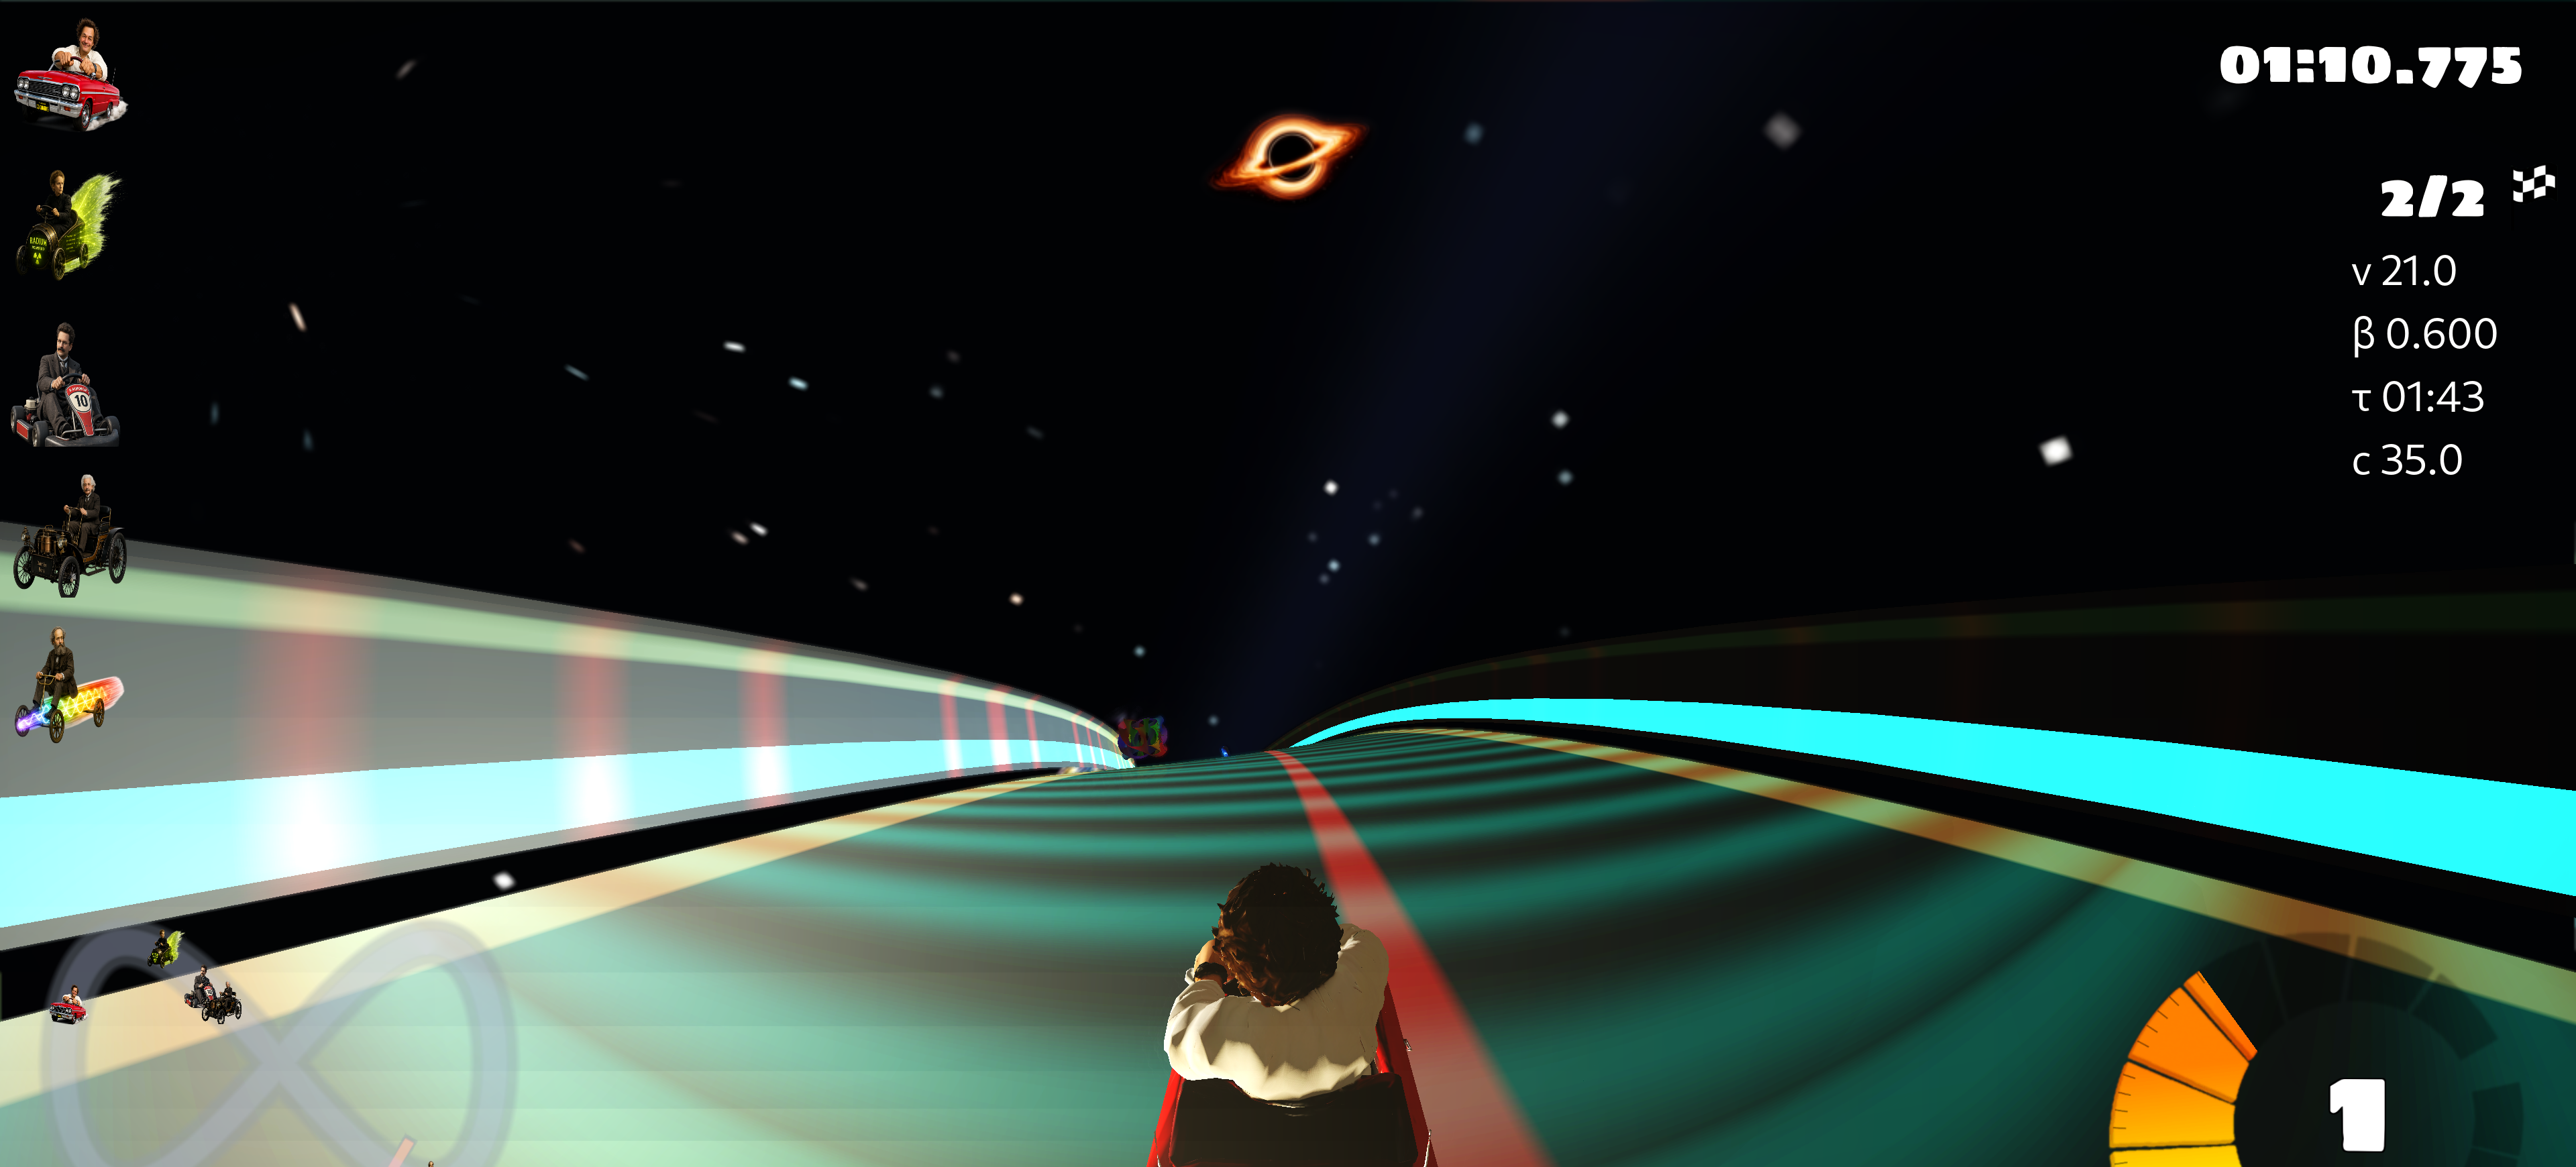
\includegraphics[width=\columnwidth]{figures/mobius_lensing.png}
\caption{A gravitational-lensing item (the glowing accretion ring overhead) seen
mid-race at $\beta=0.600$. The black-hole and wormhole power-ups render as
lensing and accretion VFX backed by shared physics constants
(Sec.~\ref{sec:game}); they are evocative effects rather than solutions of the
field equations (Sec.~\ref{sec:pedagogy}).}
\label{fig:lensing}
\end{figure}

\paragraph{Time dilation as a weapon.}
The Time Dilation power-up emits an expanding wavefront (radius
$R = 75$~u reached in $3$~s, i.e.\ a front speed of
$25$~u/s) that lowers the effective $c$ of every kart it passes,
exactly when the visible ripple reaches them; gameplay timing and the
screen-space ripple are driven from the same constants so cause and effect stay
locked together. Several other items (black hole, wormhole, anti-particle pair
production) are similarly backed by shared physics constants so that the visual
and the mechanical effect remain consistent.

% ===========================================================================
\section{Doppler and searchlight color shift}\label{sec:doppler}
% ===========================================================================

Color shift is the one place where Minkowski Kart reuses OpenRelativity's code
essentially verbatim, with attribution: the spectral
$\mathrm{RGB}\!\to\!\mathrm{XYZ}$ decomposition into Gaussian primaries, the
wavelength rescaling, and the inverse transform back to displayable RGB are taken
from OpenRelativity's color shader.\cite{Sherin2016,OpenRelativityRepo} The
relativistic Doppler/searchlight factor for a ray of view direction
$\hat{\bm{d}}$ seen by an observer with reduced velocity $\bm{\beta}$ is

\begin{equation}
s = \gamma\,(1 - \bm{\beta}\!\cdot\!\hat{\bm{d}}),
\label{eq:doppler}
\end{equation}

which blueshifts ($s<1$) objects ahead and redshifts those behind, with intensity
rescaled by $s^{-3}$ to respect the relativistic beaming of spectral radiance.
Minkowski Kart adds a circular ``scanner'' window at screen center that is left
unshifted (and rendered as a monochrome instrument readout) so the player retains
a usable view forward while the periphery shifts---an ergonomic compromise the
walking-simulator setting did not require.

% ===========================================================================
\section{Architecture and portability}\label{sec:arch}
% ===========================================================================

The relativistic state for the local observer---$\bm{\beta}$, $\gamma$, $c$, and
observer position---is gathered once per frame into an ``observer snapshot'' and
uploaded as shader uniforms shared by the OpenGL ``SP'' renderer and the Vulkan
``GE'' renderer, so the same physics drives both backends. Because the optical
transform and the gameplay queries call the identical math, on-screen appearance
and the anti-clipping ray casts agree by construction. In networked play a server
can broadcast relativity rules (baseline $c$, $\beta_{\max}$, power-up
multiplier) that override the local configuration, keeping all clients in a common
relativistic regime.

% ===========================================================================
\section{Validation}\label{sec:validation}
% ===========================================================================

Because the same routines drive both the visible distortion and the gameplay
physics, an error in the relativity module would be simultaneously a physics bug
and a rendering bug. We guard against regressions with a suite of assertions that
run at start-up in every build (\texttt{Relativity::unitTesting} in
\texttt{relativity\_math.cpp}); each checks the implementation against a
hand-computed analytic value. Representative cases are collected in
Table~\ref{tab:validation}: the Lorentz factor at $\beta=0.6$ is required to equal
$1.25$, the proper-time element $\Delta\tau=\Delta t/\gamma$ to halve at
$\gamma=2$, the longitudinal force factor $1/\gamma^3$ to reduce a unit force to
$0.512$ at $\beta=0.6$, and the velocity clamp to return exactly $\beta_{\max}c$
when fed a superluminal input. The aberration map is checked to be
distance-preserving (it only redirects rays), and to beam a forward off-axis point
toward the direction of motion, consistent with Eq.~\eqref{eq:aberration}.

\begin{table}[t]
\caption{Selected analytic checks from the start-up regression suite
(\texttt{relativity\_math.cpp}), here with $c=80$. Each is asserted to hold to
$\sim10^{-5}$ in every build.}
\label{tab:validation}
\begin{ruledtabular}
\begin{tabular}{lll}
Quantity & Input & Required value \\
\hline
$\gamma$                       & $\beta=0.6$             & $1.25$ \\
$\Delta\tau=\Delta t/\gamma$   & $\Delta t=1,\ \gamma=2$ & $0.5$ \\
$F_\parallel/\gamma^3$         & $F=100,\ \beta=0.6$     & $51.2$ \\
velocity clamp $\beta_{\max}c$ & $|\bm v|=100,\ \beta_{\max}c=78.4$ & $78.4$ \\
$|\hat{\bm d}_{\mathrm{obs}}|$ & any ray                 & $1$ (norm preserved) \\
\end{tabular}
\end{ruledtabular}
\end{table}

The model the game runs is summarized in Fig.~\ref{fig:curves}, which plots the
four speed-dependent quantities a player actually feels and sees: the time-dilation
factor $\gamma$, the proper-clock rate $1/\gamma$, the longitudinal force response
$1/\gamma^3$, and the head-on Doppler/searchlight factor $s=\gamma(1+\beta)$ of
Eq.~\eqref{eq:doppler}. The sharp upturn of $\gamma$ and the equally sharp collapse
of $1/\gamma^3$ near $\beta=1$ are the quantitative origin of the ``wall at $c$''
the player experiences: past $\beta\approx0.9$, almost no additional engine force
converts into coordinate speed.

\begin{figure}[t]
\centering
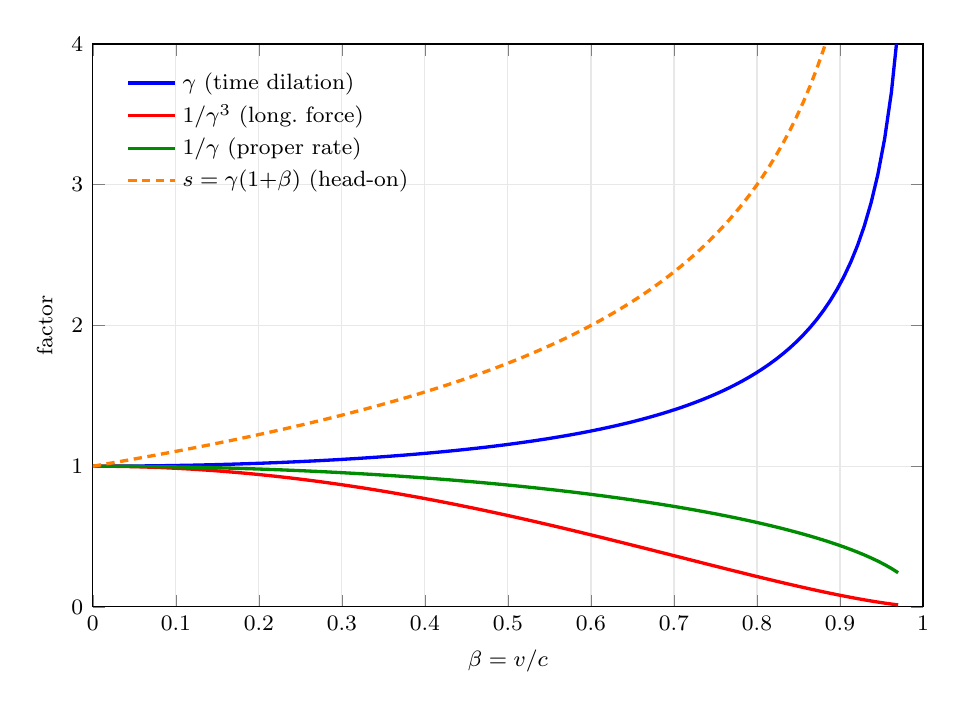
\begin{tikzpicture}
\begin{axis}[
  width=\columnwidth, height=0.72\columnwidth,
  xlabel={$\beta = v/c$}, ylabel={factor},
  domain=0:0.97, samples=120,
  xmin=0, xmax=1, ymin=0, ymax=4,
  legend pos=north west, legend cell align=left,
  legend style={font=\footnotesize, draw=none, fill=none},
  grid=both, grid style={gray!18}, tick label style={font=\footnotesize},
  label style={font=\footnotesize},
]
\addplot[very thick, blue]            {1/sqrt(1-x*x)};         \addlegendentry{$\gamma$ (time dilation)}
\addplot[very thick, red]             {(1-x*x)^(1.5)};         \addlegendentry{$1/\gamma^3$ (long.\ force)}
\addplot[very thick, green!55!black]  {sqrt(1-x*x)};           \addlegendentry{$1/\gamma$ (proper rate)}
\addplot[very thick, orange, densely dashed] {(1+x)/sqrt(1-x*x)}; \addlegendentry{$s=\gamma(1{+}\beta)$ (head-on)}
\end{axis}
\end{tikzpicture}
\caption{The speed-dependent quantities implemented by the relativity module and
verified by the checks in Table~\ref{tab:validation}. The divergence of $\gamma$
and the collapse of the longitudinal force factor $1/\gamma^3$ as $\beta\to1$ are
what make the speed of light feel like a hard ceiling during play, while the
head-on Doppler factor $s$ drives the color shift of Fig.~\ref{fig:warp}.}
\label{fig:curves}
\end{figure}

% ===========================================================================
\section{Pedagogical use and limitations}\label{sec:pedagogy}
% ===========================================================================

By placing the speed of light within reach of an everyday action---driving---the
game makes several relativistic phenomena directly manipulable: aberration and
Terrell rotation (watch an opponent appear to swing around as it overtakes),
relativistic Doppler shift, the $\gamma^3$ resistance to further acceleration,
and proper-time lag between coordinate and on-board clocks. Unlike a fixed
demonstration, the player sets $c$ and explores the continuum between the
Newtonian and ultrarelativistic limits.

The model has clear limitations, appropriate to flag for instructors. The
dynamics are special-relativistic only; the ``black hole,'' ``wormhole,'' and
``gravitational-wave'' items are evocative visual effects, not solutions of the
field equations. The optical model captures retarded position and aberration but
not relativistic shadowing or multi-bounce light transport. And the adjustable
$c$ is a single global (or per-kart) scalar, so the game does not model an
observer-dependent simultaneity beyond what the optical transform encodes. These
are reasonable simplifications for an arcade game, and each is an opening for
classroom discussion of what the simulation does and does not assert.

% ===========================================================================
\section{Conclusion}
% ===========================================================================

Minkowski Kart shows that the relativistic-rendering ideas pioneered by
OpenRelativity can be carried from a single-observer walking simulator into a
fast, many-object, competitively-played game. The three extensions that make
this possible---a per-object retarded-time-plus-aberration optical model, dynamic
GPU tessellation that resolves the nonlinear warp on arbitrary geometry, and a
playable relativistic dynamics with adjustable $c$---may be useful beyond this
particular game wherever real-time relativistic visuals must run on
externally-authored content. The source is available under the GPLv3.

\begin{acknowledgments}
We thank the SuperTuxKart contributors for the underlying engine and the MIT Game
Lab for OpenRelativity, whose physical model and color-shift code this work
builds upon.
\end{acknowledgments}

% ===========================================================================
\begin{thebibliography}{99}

\bibitem{Sherin2016}
Z.~W. Sherin, R.~Cheu, P.~Tan, and G.~Kortemeyer,
``Visualizing relativity: The OpenRelativity project,''
Am. J. Phys. \textbf{84}, 369--374 (2016).

\bibitem{OpenRelativityRepo}
MIT Game Lab, ``OpenRelativity,''
\url{https://github.com/MITGameLab/OpenRelativity} (accessed 2026).

\bibitem{Savage2007}
C.~M. Savage, A.~Searle, and L.~McCalman,
``Real Time Relativity: Exploratory learning of special relativity,''
Am. J. Phys. \textbf{75}, 791--798 (2007).

\bibitem{Kraus2008}
U.~Kraus,
``First-person visualizations of the special and general theory of relativity,''
Eur. J. Phys. \textbf{29}, 1--13 (2008).

\bibitem{Terrell1959}
J.~Terrell,
``Invisibility of the Lorentz contraction,''
Phys. Rev. \textbf{116}, 1041--1045 (1959).

\bibitem{Penrose1959}
R.~Penrose,
``The apparent shape of a relativistically moving sphere,''
Proc. Cambridge Philos. Soc. \textbf{55}, 137--139 (1959).

\bibitem{Weisskopf1960}
V.~F. Weisskopf,
``The visual appearance of rapidly moving objects,''
Phys. Today \textbf{13}(9), 24--27 (1960).

\bibitem{Hsiung1990}
P.-K. Hsiung and R.~H.~P. Dunn,
``Visualizing relativistic effects in spacetime,''
in \emph{Proceedings of the 1989 ACM/IEEE Conference on Supercomputing}
(ACM, New York, 1989), pp. 597--606.

\bibitem{Weiskopf2000}
D.~Weiskopf, U.~Kraus, and H.~Ruder,
``Searchlight and Doppler effects in the visualization of special relativity:
A corrected derivation of the transformation of radiance,''
ACM Trans. Graph. \textbf{18}, 278--292 (1999).

\bibitem{STK}
SuperTuxKart contributors, ``SuperTuxKart,''
\url{https://github.com/supertuxkart/stk-code} (accessed 2026).

\end{thebibliography}

\end{document}
